% Provenance (never printed): see sources/outline_sources.md (Year 2: interstellar
% medium, molecular clouds, gravitational collapse and the Jeans criterion, protostars
% and protostellar discs). Curves from figdata/bachelor-2/jeans.py; exercise and problem
% values in the Book 4 scratch calculator calc/ch01.py.
\chapter{The Interstellar Medium and Star Formation}\label{ch:b2:ism-star-formation}

In the constellation of Taurus, about \qty{140}{\parsec} from the Sun, a dark
patch blots out the stars behind it. Seen with a radio telescope tuned to the
lines of carbon monoxide, the patch is a cloud of cold gas some twenty
thousand times as massive as the Sun, laced with filaments; inside the densest
knots, young stars are being born, and around one of them, HL Tauri, a disc of
dust shows a pattern of bright and dark rings where planets may already be
forming. The Sun, the Earth and every atom in the rocks of this book once lay
in such a cloud. This chapter follows the matter of a planetary system from
the thin gas between the stars to a disc around a newborn star: what the
\omterm{def:b2:ism-star-formation:ism}{interstellar medium} is made of, why a cloud supported by its own heat ever
collapses, how long the collapse takes, how a star assembles its mass and
why the matter that fails to fall into it ends in a disc.

\begin{recall}
A star on the main sequence shines by fusing hydrogen into helium in its
core and holds itself up by its pressure against its own weight; its
position in the Hertzsprung--Russell diagram is set by its mass (physics,
University Year 3). A body on a closed orbit about a mass $M$ obeys Kepler's
third law, $T^2 = 4\pi^2 a^3/(GM)$ (physics, University Year 1). A black body
of temperature $T$ emits $\sigma T^4$ per unit area (physics, University
Year 2). In an ideal gas of $N$ particles the mean kinetic energy of
translation is $\tfrac32 N k_{\mathrm B} T$. The parsec,
\qty{3.086e16}{m}, is the distance unit of the Year 1 volume.
\end{recall}

\section{The matter between the stars}

Space between the stars is not empty. Near the Sun it holds on average about
one atom of hydrogen per cubic centimetre, a mass density of
\qty{2.7e-24}{g.cm^{-3}}; the air we breathe holds some $10^{19}$ times more
molecules in the same volume (\cref{exo:b2:ism-star-formation:1}). Spread over the Galaxy, this thin
matter still amounts to \qtyrange{10}{15}{\percent} of the mass of the
Galactic disc.
% ledger: ferriere:mean-density, ferriere:disc-fraction

\begin{definition}[Interstellar medium, interstellar dust]
\label{def:b2:ism-star-formation:ism}
The \emph{interstellar medium}\index{interstellar medium} is the gas and dust
that fill the space between the stars of a galaxy. \emph{Interstellar
dust}\index{interstellar dust} is the part of it in solid grains, from a few
nanometres to about a micrometre across, made of silicates, carbon compounds
and, in cold regions, ices.
\end{definition}

Its composition is the one measured in the Sun and in meteorites: by mass,
\qty{70.4}{\percent} hydrogen, \qty{28.1}{\percent} helium and
\qty{1.5}{\percent} heavier elements. Only \qtyrange{0.5}{1}{\percent} of the
mass is in dust, yet the dust holds most of some elements: the gas is poorer
than the Sun in magnesium, silicon and iron by factors of 10 to 100, because
those atoms are locked in the grains, while carbon, nitrogen and oxygen are
depleted only by factors of 1.2 to 3. The grains are the first solids of a
future planetary system; \cref{ch:b2:planet-formation-meteorites}
follows them.
% ledger: ferriere:composition, ferriere:dust-fraction, ferriere:refractory-depletion

\subsection{Five phases}

The gas is far from uniform. It comes in a few distinct states, or phases,
each with its own range of temperature and density (table below). About half
its mass is in clouds that fill only \qtyrange{1}{2}{\percent} of the volume;
the rest, warm or hot, fills the space between them.
% ledger: ferriere:disc-fraction

\begin{table}[htbp]
\centering
\small
\begin{tabular}{lll}
\hline
phase & temperature (K) & density $n$ (\unit{cm^{-3}}) \\
\hline
molecular & 10--20 & $10^2$--$10^6$ \\
cold atomic & 50--100 & 20--50 \\
warm atomic & 6000--10\,000 & 0.2--0.5 \\
warm ionised & about 8000 & 0.2--0.5 \\
hot ionised & about $10^6$ & about 0.0065 \\
\hline
\end{tabular}
\caption{The phases of the interstellar gas near the Sun; $n$ is the number
density of hydrogen nuclei.}
\label{tab:b2:ism-star-formation:phases}
% ledger: ferriere:molecular, ferriere:cold-atomic, ferriere:warm-atomic, ferriere:warm-ionized, ferriere:hot-ionized
\end{table}

The table hides a regularity. The pressure of an ideal gas is
$P = n k_{\mathrm B} T$, so the product $nT$ measures it. For the cold atomic
gas $nT$ is about $30\times75 \approx 2000$ (in \unit{K.cm^{-3}}), for the warm
atomic gas about $0.3\times8000 \approx 2400$, for the hot gas about
$0.0065\times10^6 = 6500$: within a factor of a few, the three phases that
share the space between the clouds are at the same pressure (figure below).
Where a hot and a cold gas touch at equal pressure, neither pushes the other
away; a gas that cools at constant pressure grows denser in proportion and
drops from the warm phase into the cold one. The \omterm{def:b2:ism-star-formation:molecular-cloud}{molecular clouds} reach far higher pressures, up to thousands of times more in their dense parts: they are held together by their own gravity, not by the
pressure of their surroundings.

\begin{omfigure}
\begin{tikzpicture}
\begin{axis}[omrecord, width=0.86\linewidth, height=6.4cm, xmode=log, ymode=log,
  xmin=1e-3, xmax=1e7, ymin=3, ymax=3e6,
  xlabel={density of hydrogen nuclei $n$ (\unit{cm^{-3}})}, ylabel={temperature $T$ (K)},
  tick label style={font=\scriptsize}, label style={font=\small}, clip=false,
  legend pos=north east, legend style={font=\scriptsize, draw=black!30}]
\addplot[black!45, densely dashed, domain=1e-3:1e3, samples=2] {3000/x};
\addlegendentry{$nT = \num{3000}$}
\addplot[black!60, densely dotted, thick, domain=0.1:1e5, samples=2] {3e5/x};
\addlegendentry{$nT = 3\times10^5$}
\fill[blue!45, opacity=0.6] (axis cs:1e2,10) rectangle (axis cs:1e6,20);
\fill[teal!50, opacity=0.6] (axis cs:20,50) rectangle (axis cs:50,100);
\fill[orange!55, opacity=0.6] (axis cs:0.2,6000) rectangle (axis cs:0.5,10000);
\fill[red!45, opacity=0.6] (axis cs:0.2,5714) rectangle (axis cs:0.5,11200);
\fill[violet!50, opacity=0.6] (axis cs:0.00464,7.14e5) rectangle (axis cs:0.0091,1.4e6);
\node[font=\scriptsize, anchor=south east] at (axis cs:1e6,20) {molecular clouds};
\node[font=\scriptsize, anchor=south west] at (axis cs:50,100) {cold atomic};
\node[font=\scriptsize, anchor=east, align=right] at (axis cs:0.17,8000) {warm atomic\\and warm ionised};
\node[font=\scriptsize, anchor=west] at (axis cs:0.011,1e6) {hot ionised};
\end{axis}
\end{tikzpicture}

\par\smallskip{\small The phases of the interstellar gas near the Sun (ranges of the table
above; the warm ionised and hot phases, given as single values, are drawn as boxes
a factor 1.4 wide). Along each grey line the pressure $nk_{\mathrm B}T$ is constant: the
cold, warm and hot phases lie close to the same pressure, within a factor of a few,
while the \omterm{def:b2:ism-star-formation:molecular-cloud}{molecular clouds}, bound by their own gravity, reach pressures up to thousands of times higher.
Data: Ferrière (2001).}
\end{omfigure}

Dust shows itself in three ways. It dims the light of the stars behind it,
and dims blue light more than red, so that stars seen through it look redder
than they are. It shines in the far infrared and at millimetre wavelengths,
at the temperature of a few tens of kelvins to which starlight warms it. And
it hides whatever lies inside a dense cloud from optical telescopes, which is
why star formation is observed at radio and infrared wavelengths. The gas is
traced by its lines: atomic hydrogen by its radio line at \qty{21}{cm},
molecular hydrogen, which hardly radiates when cold, by the lines of the
molecules that come with it, carbon monoxide first among them.

\section{Molecular clouds}

The coldest and densest phase is where stars form.

\begin{definition}[Molecular cloud, dense core]
\label{def:b2:ism-star-formation:molecular-cloud}
A \emph{molecular cloud}\index{molecular cloud} is a region of the
\omterm{def:b2:ism-star-formation:ism}{interstellar medium} dense and opaque enough for its hydrogen to be mostly in
molecules, \ce{H2}, shielded by dust from the ultraviolet light of the stars
that would break them; its temperature is about \qty{10}{K} to \qty{20}{K}. A
\emph{dense core}\index{dense core} is a compact condensation inside a
molecular cloud, a few tenths of a parsec across or less, with densities of
$10^4$ to $10^5$ particles per cubic centimetre, from which a single star or a
small group of stars forms.
\end{definition}

Clouds are organised in a hierarchy (table below). A dark cloud like Taurus
holds clumps, and the clumps hold cores, each level denser, smaller and more
quiet than the one above it: in a core the gas moves at a few tenths of a
kilometre per second at most, the speed of sound in gas at \qty{10}{K}. The
region of Taurus mapped in carbon monoxide holds about \num{2.4e4} solar
masses of gas; only \qtyrange{0.3}{1.2}{\percent} of it has turned into the
young stars seen there, at a rate of about eight stars every hundred thousand
years over the last three million years. Star formation is slow and wasteful.
% ledger: bt07:clouds, bt07:clumps, bt07:cores, goldsmith:taurus-mass, goldsmith:taurus-sfe, goldsmith:taurus-distance

\begin{table}[htbp]
\centering
\small
\begin{tabular}{lccc}
\hline
 & dark clouds & clumps & \omterm{def:b2:ism-star-formation:molecular-cloud}{dense cores} \\
\hline
mass (solar masses) & $10^3$--$10^4$ & 50--500 & 0.5--5 \\
size (pc) & 2--15 & 0.3--3 & 0.03--0.2 \\
mean density (\unit{cm^{-3}}) & 50--500 & $10^3$--$10^4$ & $10^4$--$10^5$ \\
gas temperature (K) & about 10 & 10--20 & 8--12 \\
examples & Taurus, Musca & --- & L1544, B68 \\
\hline
\end{tabular}
\caption{The hierarchy of a dark \omterm{def:b2:ism-star-formation:molecular-cloud}{molecular cloud}. Densities count all
particles. Data: Bergin and Tafalla (2007).}
\label{tab:b2:ism-star-formation:hierarchy}
% ledger: bt07:clouds, bt07:clumps, bt07:cores
\end{table}

Why are the clouds so cold? Gas loses energy by emitting photons that
escape, and molecules are efficient emitters: a collision lifts a carbon
monoxide molecule to a higher rotation level, the molecule falls back by
emitting a photon at millimetre wavelength, and the photon leaves the cloud,
taking the energy of the collision with it. Dust, warmed by the faint
starlight that gets in, radiates in the far infrared. The heating, by cosmic
rays and by starlight filtered through the dust, is weak; the balance settles
near \qty{10}{K}. In such gas the thermal pressure is small, and gravity can
win.

\begin{omfigure}
\begin{minipage}[c]{0.44\linewidth}
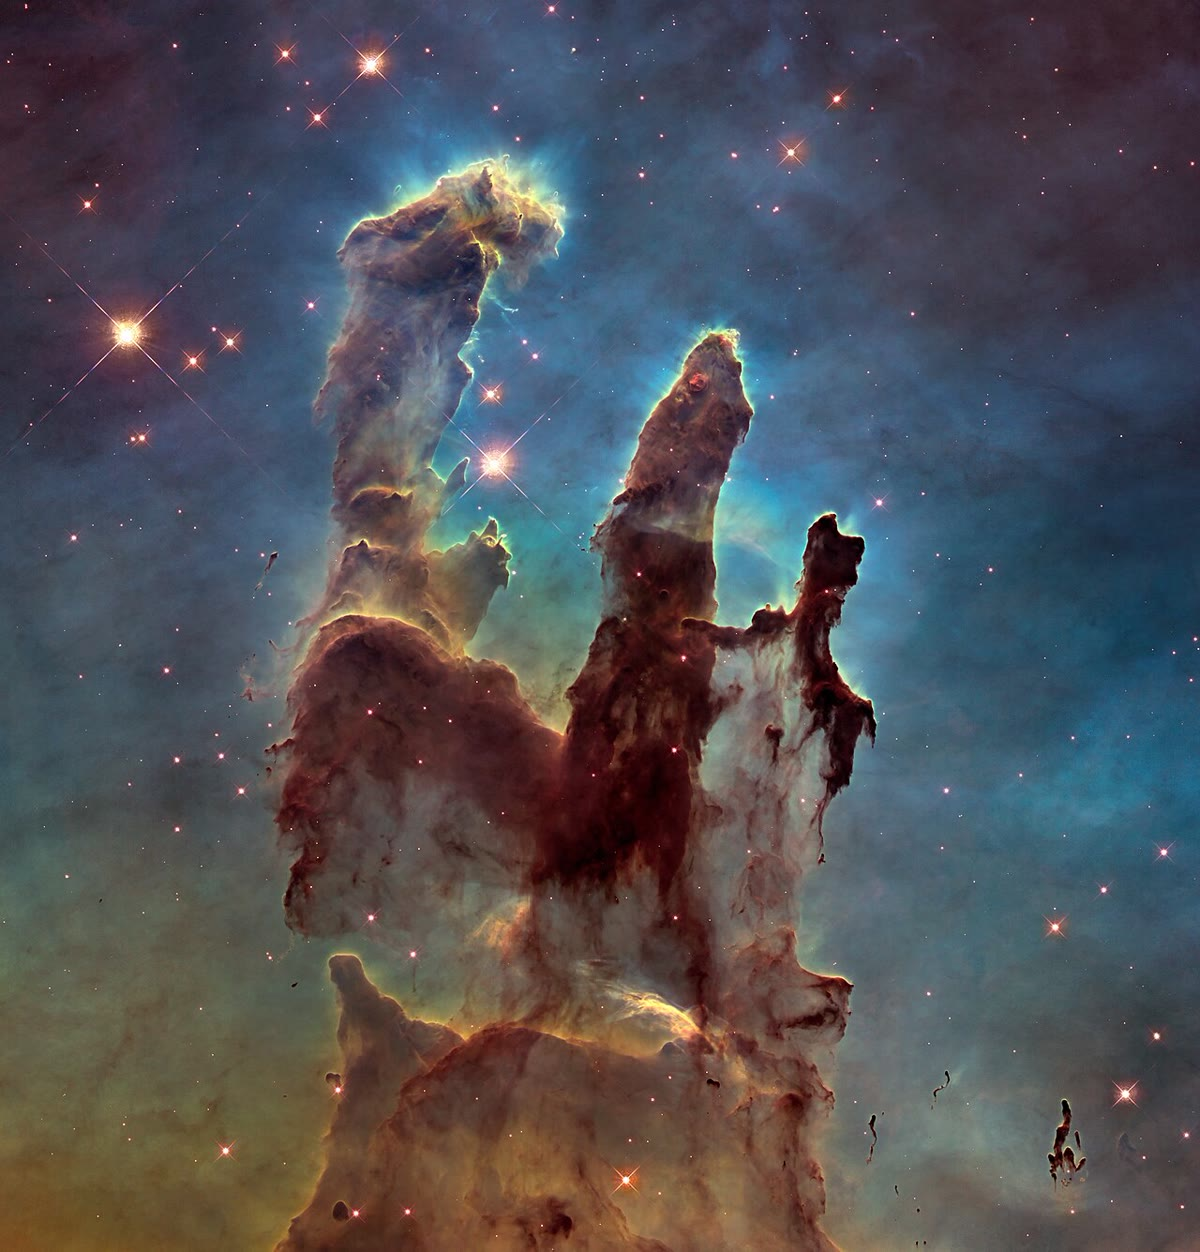
\includegraphics[width=\linewidth]{images/book4/b2-pillars-of-creation.jpg}
\end{minipage}\hfill
\begin{minipage}[c]{0.52\linewidth}
{\small The ``Pillars of Creation'' in the Eagle Nebula, imaged by the Hubble
Space Telescope in visible light. The columns are cold, dense molecular gas and
dust, light-years long, eroded and lit from above by the ultraviolet light of
massive young stars outside the picture; the dust makes them opaque. Small
condensations at their tips are forming stars. NASA, ESA and the Hubble
Heritage Team (STScI/AURA), public domain.}
\end{minipage}
\end{omfigure}

\section{Gravitational collapse}

A cloud is a balance between two energies: the thermal energy of its gas,
which pushes outward, and its gravitational energy, which pulls inward. The
second grows faster with mass than the first; above a certain mass, gravity
wins.

\begin{proposition}[Gravitational energy of a uniform sphere]
\label{prop:b2:ism-star-formation:grav-energy}
A sphere of uniform density, of mass $M$ and radius $R$, has the
gravitational potential energy
\[
  U = -\frac{3}{5}\,\frac{G M^2}{R}.
\]
\end{proposition}

\begin{proof}
Build the sphere shell by shell. When its radius is $r$ it has the mass
$m(r) = M r^3/R^3$; bringing a shell of thickness $\mathrm dr$, of mass
$\mathrm dm = 3M r^2\,\mathrm dr/R^3$, from infinity to its surface releases
the energy $G m(r)\,\mathrm dm/r$, because a sphere attracts outside it as if
its mass were at its centre (the shell theorem, physics). Hence
\[
  U = -\int_0^R \frac{G}{r}\,\frac{M r^3}{R^3}\,\frac{3 M r^2}{R^3}\,\mathrm dr
    = -\frac{3 G M^2}{R^6}\int_0^R r^4\,\mathrm dr = -\frac{3}{5}\,\frac{G M^2}{R}.
  \qedhere
\]
\end{proof}

A self-gravitating body in equilibrium obeys the virial theorem: averaged
over time, twice its kinetic energy plus its gravitational energy is zero,
$2K + U = 0$ (physics, University Year 3, where it is derived from the
equations of motion). For a cloud at rest, $K$ is the thermal energy of its
particles. If $2K > |U|$ the gas expands; if $2K < |U|$ gravity has no
equilibrium to oppose it and the cloud contracts.

\begin{proposition}[Jeans criterion]\label{prop:b2:ism-star-formation:jeans}
A uniform, isothermal cloud of temperature $T$ and density $\rho$, made of
particles of mean mass $\mu m_u$, collapses under its own gravity if its mass
exceeds the \emph{\omterm{def:b2:ism-star-formation:jeans}{Jeans mass}}
\[
  M_J = \left(\frac{5 k_{\mathrm B} T}{G\mu m_u}\right)^{3/2}
        \left(\frac{3}{4\pi\rho}\right)^{1/2},
\]
or equivalently if its radius exceeds the \emph{\omterm{def:b2:ism-star-formation:jeans}{Jeans length}}
\[
  R_J = \left(\frac{15 k_{\mathrm B} T}{4\pi G\mu m_u\,\rho}\right)^{1/2}.
\]
This is the \emph{Jeans criterion}\index{Jeans criterion}.
\end{proposition}

\begin{proof}
The cloud holds $N = M/(\mu m_u)$ particles, with the thermal energy
$K = \tfrac32 N k_{\mathrm B}T = \tfrac32 M k_{\mathrm B}T/(\mu m_u)$. By
\cref{prop:b2:ism-star-formation:grav-energy}, it collapses if
$2K < \tfrac35 GM^2/R$, that is
\[
  \frac{3 M k_{\mathrm B} T}{\mu m_u} < \frac{3}{5}\,\frac{G M^2}{R}
  \iff M > \frac{5 k_{\mathrm B} T}{G \mu m_u}\, R .
\]
Eliminate $R$ with $M = \tfrac43\pi R^3\rho$, that is $R = (3M/4\pi\rho)^{1/3}$:
$M^{2/3} > \frac{5 k_{\mathrm B}T}{G\mu m_u}\,(3/4\pi\rho)^{1/3}$, and raising
both sides to the power $3/2$ gives $M > M_J$. Eliminating $M$ instead,
$\tfrac43\pi R^3\rho > 5 k_{\mathrm B}T R/(G\mu m_u)$ gives $R^2 > 15
k_{\mathrm B}T/(4\pi G\mu m_u\rho)$, that is $R > R_J$.
\end{proof}

\begin{definition}[Jeans mass, Jeans length]\label{def:b2:ism-star-formation:jeans}
The \emph{Jeans mass}\index{Jeans mass} $M_J$ and the \emph{Jeans
length}\index{Jeans length} $R_J$ of a gas of given temperature and density
are the mass and the radius above which a uniform sphere of that gas
collapses under its own gravity (\cref{prop:b2:ism-star-formation:jeans}).
\end{definition}

The \omterm{def:b2:ism-star-formation:jeans}{Jeans mass} grows as $T^{3/2}$ and falls as $\rho^{-1/2}$: cold, dense gas
collapses most easily. In a \omterm{def:b2:ism-star-formation:molecular-cloud}{molecular cloud} the mean mass per particle is
$\mu = 2.33$ atomic mass units, molecular hydrogen with one helium atom for
about every five molecules. At \qty{10}{K} and $10^4$ particles per cubic
centimetre, $\rho = \mu m_u n = \qty{3.87e-17}{kg.m^{-3}}$ and
$M_J = 5.5$ solar masses, inside a \omterm{def:b2:ism-star-formation:jeans}{Jeans length} of \qty{0.13}{\parsec}:
the mass and the size of a \omterm{def:b2:ism-star-formation:molecular-cloud}{dense core}. At the mean density of a dark cloud,
$100$ particles per cubic centimetre, the \omterm{def:b2:ism-star-formation:jeans}{Jeans mass} is ten times larger, 55
solar masses, and a cloud of \num{24000} solar masses like Taurus contains
hundreds of them (figure below).
% ledger: kauffmann:mu, nist:u, const:kB, const:G, sun:mass, goldsmith:taurus-mass

\begin{omfigure}
\begin{tabular}{@{}c@{\hspace{3mm}}c@{}}
\begin{tikzpicture}
\begin{axis}[omrecord, width=0.455\linewidth, height=6.0cm, xmode=log, ymode=log,
  xmin=10, xmax=1e7, ymin=0.05, ymax=1e4,
  xlabel={$n$ (\unit{cm^{-3}})}, ylabel={Jeans mass (solar masses)},
  tick label style={font=\scriptsize}, label style={font=\small},
  legend style={font=\scriptsize, at={(0.97,0.97)}, anchor=north east, draw=none, fill=white, fill opacity=0.85}]
\fill[blue!12] (axis cs:1e4,0.5) rectangle (axis cs:1e5,5);
\node[font=\scriptsize, blue!50!black, anchor=north east] at (axis cs:1e5,0.5) {dense cores};
\addplot[very thick, blue!70!black] table[x=n, y=MJ10] {figdata/out/bachelor-2-jeans-jeans.dat};
\addlegendentry{\qty{10}{K}}
\addplot[very thick, orange!80!black] table[x=n, y=MJ20] {figdata/out/bachelor-2-jeans-jeans.dat};
\addlegendentry{\qty{20}{K}}
\addplot[very thick, red!75!black] table[x=n, y=MJ50] {figdata/out/bachelor-2-jeans-jeans.dat};
\addlegendentry{\qty{50}{K}}
\end{axis}
\end{tikzpicture}
&
\begin{tikzpicture}
\begin{axis}[omrecord, width=0.455\linewidth, height=6.0cm, xmode=log, ymode=log,
  xmin=10, xmax=1e7, ymin=0.01, ymax=20,
  xlabel={$n$ (\unit{cm^{-3}})}, ylabel={free-fall time (Myr)},
  tick label style={font=\scriptsize}, label style={font=\small}]
\addplot[very thick, black!70] table[x=n, y=tff_Myr] {figdata/out/bachelor-2-jeans-tff.dat};
\fill[blue!12] (axis cs:1e4,0.05) rectangle (axis cs:1e5,0.5);
\addplot[very thick, black!70] table[x=n, y=tff_Myr] {figdata/out/bachelor-2-jeans-tff.dat};
\node[font=\scriptsize, blue!50!black, anchor=north] at (axis cs:3.2e4,0.05) {cores};
\end{axis}
\end{tikzpicture}
\\[2pt]
{\small (a) \omterm{def:b2:ism-star-formation:jeans}{Jeans mass}} & {\small (b) \omterm{def:b2:ism-star-formation:free-fall}{free-fall time}}
\end{tabular}

\par\smallskip{\small (a) The \omterm{def:b2:ism-star-formation:jeans}{Jeans mass} against the density of particles for three
temperatures ($\mu = 2.33$). The shaded box marks the masses and densities of
observed \omterm{def:b2:ism-star-formation:molecular-cloud}{dense cores}: at \qty{10}{K} their mass is close to the \omterm{def:b2:ism-star-formation:jeans}{Jeans mass}. (b) The
\omterm{def:b2:ism-star-formation:free-fall}{free-fall time} of \cref{prop:b2:ism-star-formation:free-fall}: a third of a million
years at $10^4$ particles per cubic centimetre, ten times longer at $10^2$.}
\end{omfigure}

A cloud that starts to collapse grows denser, and its \omterm{def:b2:ism-star-formation:jeans}{Jeans mass} falls as
$\rho^{-1/2}$ while it stays cold, which it does as long as it can radiate the
heat of compression. Pieces of the cloud then become unstable on their own
and collapse separately: the cloud \emph{fragments}. This is why stars form
in groups and why their masses are small compared with the clouds that make
them. Fragmentation stops when the gas becomes too dense to let its radiation
escape: the heat of compression is trapped, the temperature rises, and the
\omterm{def:b2:ism-star-formation:jeans}{Jeans mass} stops falling.

How long does a collapse take? If pressure is negligible, each shell of the
cloud falls freely towards the centre.

\begin{proposition}[Free-fall time]\label{prop:b2:ism-star-formation:free-fall}
A uniform sphere of density $\rho$, initially at rest and without pressure,
collapses to its centre in the time
\[
  t_{\mathrm{ff}} = \left(\frac{3\pi}{32\,G\rho}\right)^{1/2},
\]
independent of its radius.
\end{proposition}

\begin{proof}
Consider a particle at rest at the distance $R$ from the centre, on the
surface of the sphere. The shells inside it fall faster or with it, never
behind, so the mass $M = \tfrac43\pi R^3\rho$ that attracts it stays the same
all the way. Its path is a degenerate Kepler orbit: an ellipse flattened into
a straight segment, with its far end at $R$ and the centre of attraction at
its other end, so its semi-major axis is $a = R/2$. Falling from the far end
to the centre takes half a period; by Kepler's third law
\[
  t_{\mathrm{ff}} = \frac12\cdot 2\pi\sqrt{\frac{(R/2)^3}{GM}}
  = \pi\sqrt{\frac{R^3}{8\,G\cdot\frac43\pi R^3\rho}}
  = \sqrt{\frac{3\pi}{32\,G\rho}} .
\]
$R$ cancels: every shell of a uniform sphere arrives at the centre at the same
moment.
\end{proof}

\begin{definition}[Free-fall time]\label{def:b2:ism-star-formation:free-fall}
The \emph{free-fall time}\index{free-fall time} of a gas of density $\rho$ is
$t_{\mathrm{ff}} = (3\pi/32G\rho)^{1/2}$, the time a uniform sphere of that
density would take to collapse under its own gravity alone.
\end{definition}

For a \omterm{def:b2:ism-star-formation:molecular-cloud}{dense core} of $10^4$ particles per cubic centimetre the \omterm{def:b2:ism-star-formation:free-fall}{free-fall time}
is \qty{0.34}{Myr}; for a whole dark cloud of $10^2$, \qty{3.4}{Myr}. If every
\omterm{def:b2:ism-star-formation:molecular-cloud}{molecular cloud} of the Galaxy collapsed in a \omterm{def:b2:ism-star-formation:free-fall}{free-fall time} and turned into
stars, the Galaxy would form stars far faster than it does: in Taurus, the gas actually turned
into stars over the last three million years is about one per cent of the cloud. The
clouds are held back, by turbulent motions and by magnetic fields that the
ionised fraction of the gas drags along, and most of their gas is dispersed by
the winds and light of the first massive stars before it can collapse: hence
the low efficiency measured in Taurus.
% ledger: bt07:tff

\begin{history}[James Jeans]
James Jeans (1877--1946) published in 1902 the analysis of the stability of a
gas under its own gravity from which the \omterm{def:b2:ism-star-formation:jeans}{Jeans mass} and length descend. He
studied the growth of small density waves in an infinite uniform gas and
found that waves longer than a critical length are not opposed by pressure
but grow: the gas breaks into condensations of about that size. His critical
length differs from the radius found above by a numerical factor only; the
physics, gravity against thermal pressure, is the same.
\end{history}

\section{Protostars}

The collapse of a core is not uniform. The centre, slightly denser, falls
first; a small, dense, hot object forms there and grows by swallowing the gas
that keeps raining onto it.

\begin{definition}[Protostar]\label{def:b2:ism-star-formation:protostar}
A \emph{protostar}\index{protostar} is a star in formation that is still
gaining most of its mass by accretion of the gas of its parent core; it
shines by the energy that the falling gas releases, not by nuclear fusion.
\end{definition}

How fast does a \omterm{def:b2:ism-star-formation:protostar}{protostar} grow? A core near collapse holds about a \omterm{def:b2:ism-star-formation:jeans}{Jeans mass}
and falls in about a \omterm{def:b2:ism-star-formation:free-fall}{free-fall time}, so the mass arrives at a rate of order
$M_J/t_{\mathrm{ff}}$.

\begin{proposition}[Accretion rate of a protostar]
\label{prop:b2:ism-star-formation:accretion}
Let $c_s = (k_{\mathrm B}T/\mu m_u)^{1/2}$ be the isothermal speed of sound
of the gas of a core. The ratio of the \omterm{def:b2:ism-star-formation:jeans}{Jeans mass} to the \omterm{def:b2:ism-star-formation:free-fall}{free-fall time} does
not depend on the density, and
\[
  \frac{M_J}{t_{\mathrm{ff}}} \approx 10\,\frac{c_s^3}{G}:
\]
a \omterm{def:b2:ism-star-formation:protostar}{protostar} grows at a rate of order $c_s^3/G$, set by the temperature of its
core alone.
\end{proposition}

\begin{proof}
With $k_{\mathrm B}T/(\mu m_u) = c_s^2$, $M_J = 5^{3/2}\,c_s^3\,G^{-3/2}
(3/4\pi\rho)^{1/2}$ and $t_{\mathrm{ff}} = (3\pi/32)^{1/2}(G\rho)^{-1/2}$, so
\[
  \frac{M_J}{t_{\mathrm{ff}}} = 5^{3/2}\left(\frac{3}{4\pi}\right)^{1/2}
  \left(\frac{32}{3\pi}\right)^{1/2}\frac{c_s^3}{G}
  = 11.18\times0.489\times1.84\,\frac{c_s^3}{G} \approx 10\,\frac{c_s^3}{G},
\]
in which $\rho$ has cancelled. The factor depends on the shape of the core;
models of cores whose density falls off outward, as observed, give rates
nearer to $c_s^3/G$ itself.
\end{proof}

At \qty{10}{K}, $c_s = \qty{0.19}{km.s^{-1}}$ and $c_s^3/G$ is
\num{1.6e-6} solar masses per year: a star like the Sun assembles in about
\num{600000} years, a time comparable to the \omterm{def:b2:ism-star-formation:free-fall}{free-fall time} of its core.
In a warmer core, at \qty{20}{K}, the rate is $2^{3/2} = 2.8$ times higher.

\begin{omfigure}
\begin{tikzpicture}[font=\scriptsize]
% panel 1: core
\begin{scope}
\shade[inner color=gray!70, outer color=gray!10] (0,0) circle (1.0);
\node[align=center] at (0,-1.45) {(1) dense core\\$\sim\qty{0.1}{pc}$, \qty{10}{K}};
\end{scope}
% panel 2: collapse with infall arrows
\begin{scope}[xshift=3.0cm]
\shade[inner color=gray!80, outer color=gray!10] (0,0) circle (0.9);
\foreach \a in {0,45,...,315} \draw[-{Stealth[length=1.6mm]}, black!70] (\a:0.85) -- (\a:0.3);
\fill[orange!90!red] (0,0) circle (0.07);
\node[align=center] at (0,-1.45) {(2) collapse\\$t_{\mathrm{ff}} \sim \qty{0.1}{Myr}$};
\end{scope}
% panel 3: protostar with disc and outflow
\begin{scope}[xshift=6.0cm]
\fill[gray!25] (0,0) ellipse (0.9 and 0.6);
\fill[brown!55] (0,0) ellipse (0.75 and 0.12);
\fill[orange!90!red] (0,0) circle (0.08);
\fill[blue!25] (0,0.1) -- (-0.22,0.95) -- (0.22,0.95) -- cycle;
\fill[blue!25] (0,-0.1) -- (-0.22,-0.95) -- (0.22,-0.95) -- cycle;
\node[align=center] at (0,-1.45) {(3) protostar, disc\\and outflow, $\sim\qty{0.5}{Myr}$};
\end{scope}
% panel 4: T Tauri with disc
\begin{scope}[xshift=9.0cm]
\fill[brown!55] (0,0) ellipse (0.85 and 0.1);
\fill[yellow!80!orange] (0,0) circle (0.1);
\draw[blue!40, thick] (0,0.15) -- (0,0.6); \draw[blue!40, thick] (0,-0.15) -- (0,-0.6);
\node[align=center] at (0,-1.45) {(4) T Tauri star\\and disc, 1--\qty{5}{Myr}};
\end{scope}
% panel 5: planetary system
\begin{scope}[xshift=12.0cm]
\fill[yellow!80!orange] (0,0) circle (0.12);
\foreach \r in {0.3,0.5,0.8} \draw[black!40] (0,0) ellipse ({\r} and {0.4*\r});
\fill (0.3,0) circle (0.03); \fill (-0.5,0.03) circle (0.035); \fill (0.8,0.05) circle (0.06);
\node[align=center] at (0,-1.45) {(5) main-sequence\\star and planets};
\end{scope}
\foreach \x in {1.4,4.4,7.4,10.4} \draw[-{Stealth}, thick, black!60] (\x,0) -- (\x+0.25,0);
\end{tikzpicture}

\par\smallskip{\small From a \omterm{def:b2:ism-star-formation:molecular-cloud}{dense core} to a planetary system (schematic, not to scale).
(1) A cold core near the \omterm{def:b2:ism-star-formation:jeans}{Jeans mass}. (2) Its centre collapses first and a \omterm{def:b2:ism-star-formation:protostar}{protostar}
forms. (3) The \omterm{def:b2:ism-star-formation:protostar}{protostar} grows by accretion through a disc, while a \omterm{def:b2:ism-star-formation:t-tauri}{bipolar outflow}
clears gas along the rotation axis. (4) The envelope gone, a \omterm{def:b2:ism-star-formation:t-tauri}{T Tauri star}, still
contracting, is surrounded by its disc. (5) The disc has dispersed; what remains of
its solids are planets. Times from the free-fall and accretion estimates of the text
and from the disc lifetimes of the last section.}
\end{omfigure}

While it accretes, the \omterm{def:b2:ism-star-formation:protostar}{protostar} shines by the energy of the falling gas. Once
the envelope is used up, it keeps shining, still without fusion, by
contracting.

\begin{proposition}[Contraction powers a young star]
\label{prop:b2:ism-star-formation:contraction}
A self-gravitating gas sphere in equilibrium that contracts slowly radiates
half of the gravitational energy it releases and keeps the other half as heat:
it grows hotter while it loses energy.
\end{proposition}

\begin{proof}
In equilibrium the virial theorem gives $2K + U = 0$, so the total energy is
$E = K + U = U/2$. If the radius shrinks, $U$ decreases by some amount
$\Delta < 0$; then $E$ changes by $\Delta/2$, which is the energy radiated
away, and $K = -U/2$ changes by $-\Delta/2 > 0$: the thermal energy, and so
the temperature, rise by the other half.
\end{proof}

\begin{definition}[Kelvin--Helmholtz time scale]\label{def:b2:ism-star-formation:kh-time}
The \emph{Kelvin--Helmholtz time scale}\index{Kelvin--Helmholtz time scale}
of a star of mass $M$, radius $R$ and luminosity $L$ is
$t_{\mathrm{KH}} = GM^2/(RL)$, the order of magnitude of the time for which
contraction alone can supply its luminosity.
\end{definition}

For the present Sun, $t_{\mathrm{KH}} = \qty{31}{Myr}$: far shorter than its
age, which is why the Sun must burn hydrogen. For a young star of one solar
mass, twice the Sun's radius and twice its luminosity, it is \qty{8}{Myr}
(\cref{exo:b2:ism-star-formation:6}). Contraction ends when the centre becomes hot enough for hydrogen fusion to
supply the luminosity: the star arrives on the main sequence (recall).
% ledger: sun:mass, sun:R, sun:L, const:G

\begin{definition}[T Tauri star, bipolar outflow]\label{def:b2:ism-star-formation:t-tauri}
A \emph{T Tauri star}\index{T Tauri star} is a young star of less than about
two solar masses that has shed its envelope and become visible but has not
yet reached the main sequence: it shines by contraction, varies in
brightness, and is usually surrounded by a disc from which it still
accretes. A \emph{bipolar outflow}\index{bipolar outflow} is a pair of fast
jets or winds of gas ejected by a young star in opposite directions along the
rotation axis of its disc.
\end{definition}

Outflows carry away part of the angular momentum of the gas that the disc
feeds to the star, and they clear the envelope along the axis; the star of
HL Tauri, at the end of its protostellar stage, drives a highly collimated
one.
% ledger: alma:hltau

\section{Discs}

A \omterm{def:b2:ism-star-formation:molecular-cloud}{dense core} turns, slowly: across a core the gas velocity changes by a few
tenths of a kilometre per second per parsec. As the core collapses, its
angular momentum is conserved, and the slow rotation becomes fast.

\begin{proposition}[Centrifugal radius]\label{prop:b2:ism-star-formation:centrifugal}
Gas of specific angular momentum $j$ (angular momentum per unit mass)
falling towards a mass $M$ cannot reach the centre: it settles on a circular
orbit of radius
\[
  r_c = \frac{j^2}{G M}.
\]
\end{proposition}

\begin{proof}
Without friction the angular momentum of the falling gas is conserved, so at
the distance $r$ its rotation speed is $v = j/r$. The gas can circle at $r$ if
gravity supplies exactly the centripetal acceleration,
$GM/r^2 = v^2/r = j^2/r^3$, that is at $r = j^2/(GM)$. Closer in, the
centripetal acceleration needed, $j^2/r^3$, exceeds the pull of gravity, and
the gas cannot go further.
\end{proof}

Gas falling along the rotation axis has little angular momentum and goes
straight to the star; gas falling in the equatorial plane keeps its
rotation. Gas falling from opposite sides along different paths collides
above and below the equatorial plane, loses its vertical motion, and
collects into a thin rotating disc of radius about $r_c$. For a core of
\qty{0.1}{pc} turning once in some twenty million years, $r_c$ is a few
hundred astronomical units (\cref{exo:b2:ism-star-formation:11}): the size of the observed discs.

\begin{definition}[Protoplanetary disc]\label{def:b2:ism-star-formation:disc}
A \emph{protoplanetary disc}\index{protoplanetary disc} (or
\emph{protostellar disc}\index{protostellar disc}) is the flattened disc of
gas and dust in nearly Keplerian rotation around a young star, made of the
matter of its parent core that kept too much angular momentum to fall onto the
star; planets form in it.
\end{definition}

\begin{omfigure}
\begin{minipage}[c]{0.44\linewidth}
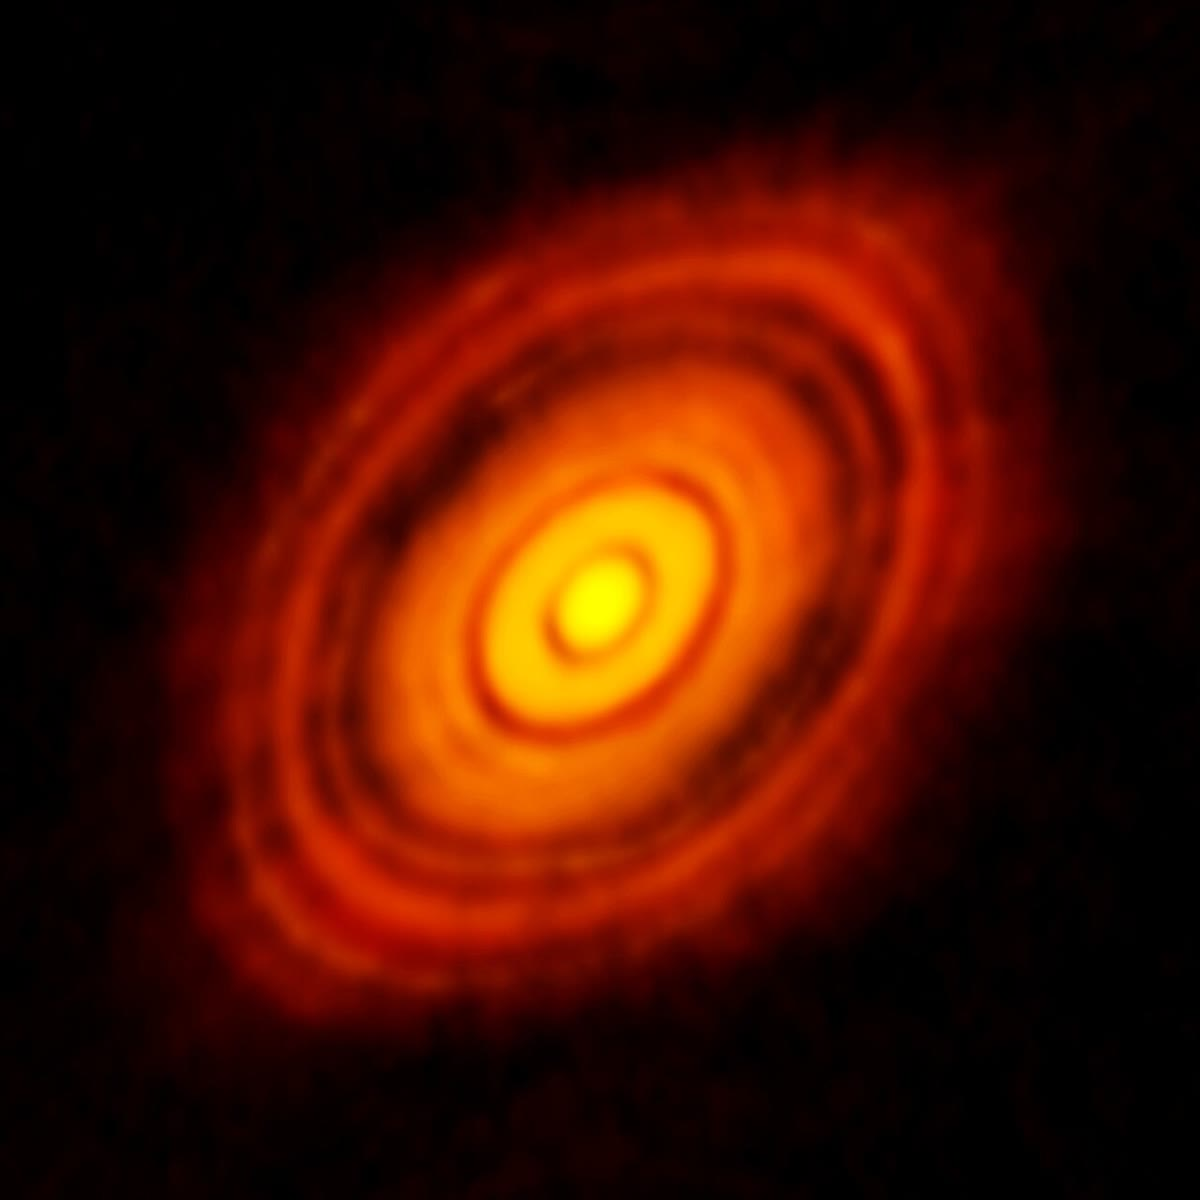
\includegraphics[width=\linewidth]{images/book4/b2-hl-tau-alma.jpg}
\end{minipage}\hfill
\begin{minipage}[c]{0.52\linewidth}
{\small The disc of the young star HL Tauri, \qty{140}{pc} away in Taurus, imaged
by the ALMA interferometer at a wavelength of about one millimetre, where cold
dust shines. The disc, about \qty{120}{au} in radius and seen tilted by
\ang{47}, shows bright and dark rings a few astronomical units wide; the
system is at most one or two million years old, and the rings are read as the
first signs of planets clearing their paths. ALMA (ESO/NAOJ/NRAO), CC BY 4.0.}
\end{minipage}
% ledger: alma:hltau
\end{omfigure}

The disc is heated by the star. A grain at the distance $r$ absorbs starlight
over its cross-section and radiates over its whole surface.

\begin{proposition}[Temperature of a grain in starlight]
\label{prop:b2:ism-star-formation:grain}
A small grain behaving as a black body, at the distance $r$ from a star of
luminosity $L$ and in sunlight on one side only, settles at the temperature
\[
  T = \left(\frac{L}{16\pi\sigma r^2}\right)^{1/4},
\]
which falls off as $r^{-1/2}$.
\end{proposition}

\begin{proof}
A spherical grain of radius $a$ intercepts the power $\pi a^2\,L/(4\pi r^2)$
and, at the temperature $T$, radiates $4\pi a^2\sigma T^4$ over its surface.
At equilibrium the two are equal: $T^4 = L/(16\pi\sigma r^2)$; $a$ cancels.
\end{proof}

At \qty{1}{au} from a star like the Sun the grain is at \qty{278}{K}; at
\qty{5.2}{au}, where Jupiter orbits, at \qty{122}{K}. Water ice condenses where
the grains are colder than about \qty{180}{K} (the condensation temperatures are
those of \cref{ch:b2:planet-formation-meteorites}), that is beyond about
\qty{2.4}{au}: the first sign of the boundary, the snow line, that separates
rocky from icy planets. A real disc is opaque, and its midplane is shielded from direct starlight; the
proposition gives the right order of magnitude and the right slope for the
surface layers that the star sees.
% ledger: lodders:tc-table

Discs do not last. Infrared excess, the glow of warm dust above what the star
alone would emit, reveals whether a star still has a disc. Counting the stars
with such an excess in clusters of different ages gives the fraction of stars
that keep their disc as a function of time (figure below): most stars have one
at birth, half have lost it by about three million years, and almost none
keeps one beyond six. Gas giants, which must gather their gas from the disc,
have to form within these few million years.
% ledger: haisch:disc-fractions, haisch:disc-lifetime

\begin{omfigure}
\begin{tikzpicture}
\begin{axis}[omrecord, width=0.8\linewidth, height=5.6cm, xmin=0, xmax=8.5, ymin=0, ymax=1.05,
  xlabel={cluster age (Myr)}, ylabel={fraction of stars with a disc},
  tick label style={font=\scriptsize}, label style={font=\small}, clip=false]
\addplot[thick, black!55, densely dashed] table[x=age, y=frac] {figdata/out/bachelor-2-jeans-discfit.dat};
\addplot[only marks, mark=*, mark size=1.8pt, blue!70!black,
  error bars/.cd, y dir=both, y explicit]
  table[x=age, y=frac, y error=err, restrict x to domain=0:10] {figdata/out/bachelor-2-jeans-discs.dat};
\node[font=\scriptsize, anchor=north west] at (axis cs:0.05,0.74) {NGC 2024};
\node[font=\scriptsize, anchor=south west] at (axis cs:1.55,0.86) {Trapezium};
\node[font=\scriptsize, anchor=south west] at (axis cs:2.35,0.71) {IC 348};
\node[font=\scriptsize, anchor=south west] at (axis cs:3.3,0.56) {NGC 2264};
\node[font=\scriptsize, anchor=south west] at (axis cs:5.1,0.15) {NGC 2362};
\node[font=\scriptsize, anchor=north east] at (axis cs:8.4,0.98) {(NGC 1960, \qty{30}{Myr}: $0.03$)};
\end{axis}
\end{tikzpicture}

\par\smallskip{\small Fraction of the stars of young clusters that show the infrared
excess of a disc, against the age of the cluster (with its error), from Haisch, Lada
and Lada (2001). The dashed line is the least-squares straight line through the five
youngest clusters: it reaches $0.5$ at \qty{3.0}{Myr} and zero at \qty{6.1}{Myr}
(\cref{exo:b2:ism-star-formation:12}).}
\end{omfigure}

\begin{inthelab}[Seeing through the dust with radio waves]
\begin{minipage}[t]{0.55\linewidth}\vspace{0pt}
Cold gas and dust are invisible to optical telescopes but shine at millimetre
wavelengths, where the atmosphere is transparent only above high, dry sites. A
radio dish of the size of a house resolves little at such wavelengths, so
astronomers combine many: in an interferometer each pair of antennas, separated
by a baseline, measures one component of the brightness pattern of the sky, and
a computer assembles the image from the hundreds of pairs that some thirty antennas make. The resolution is that of
a single telescope as wide as the longest baseline: with antennas spread over
\qty{15}{km}, the HL Tauri disc was imaged in detail of a few astronomical units at
\qty{140}{pc}. Operators move the antennas on transporters between configurations,
and the correlator combines their signals in real time.
\end{minipage}\hfill
\begin{minipage}[t]{0.42\linewidth}\vspace{0pt}
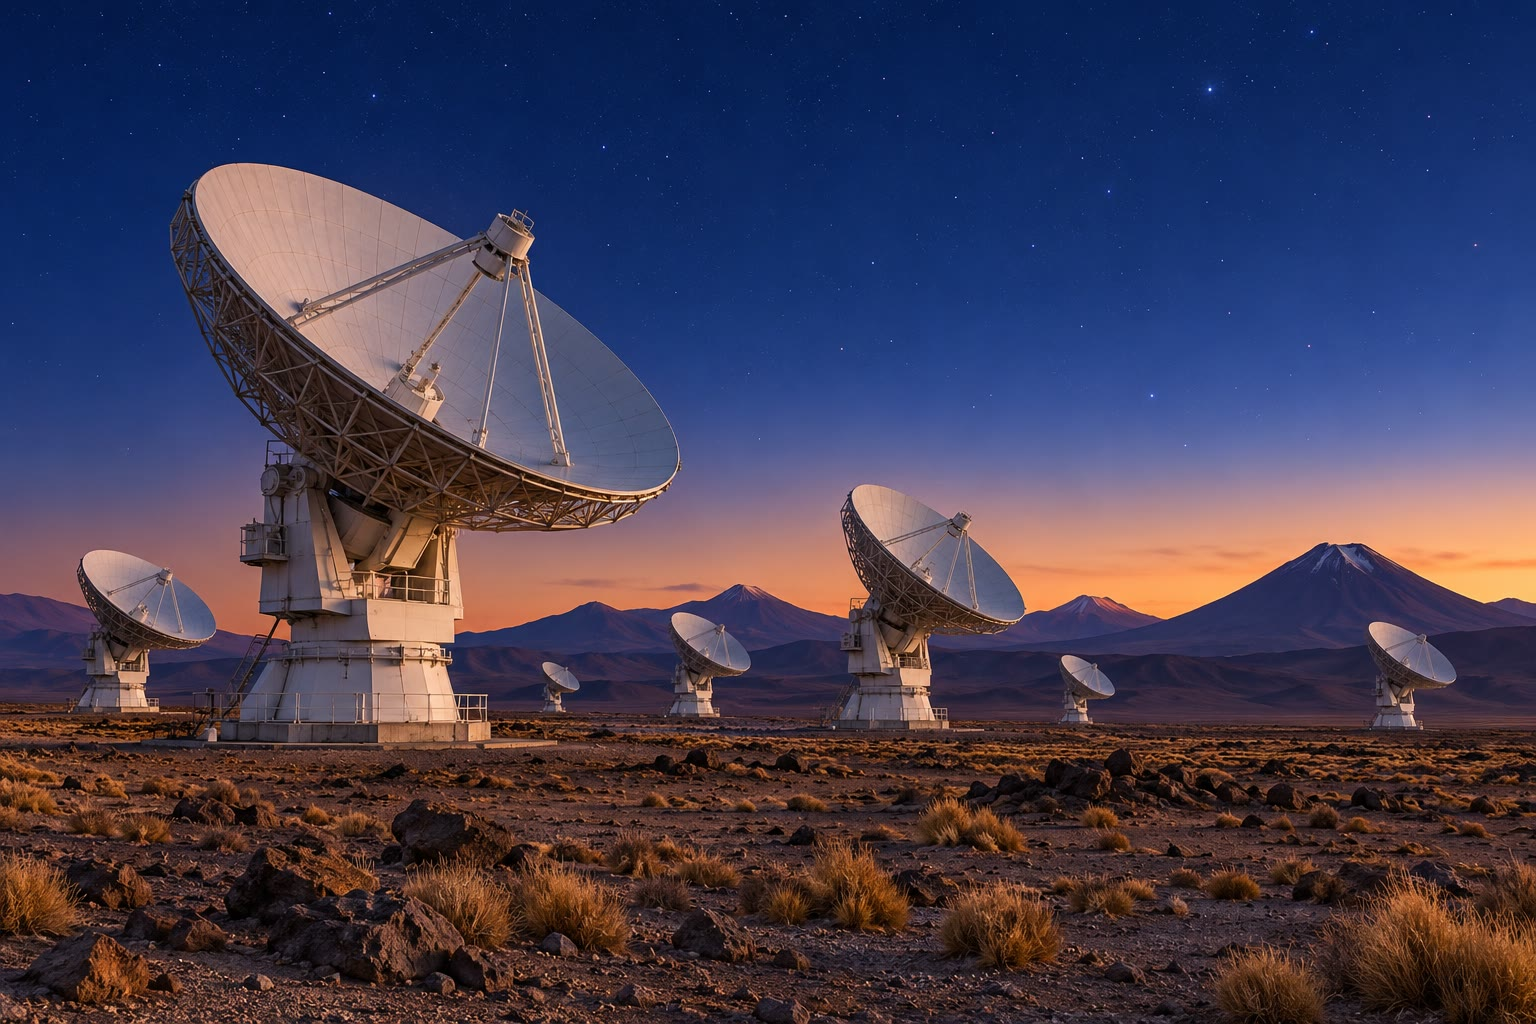
\includegraphics[width=\linewidth]{images/book4/ai/b2-radio-array.jpg}

{\scriptsize An array of radio antennas on a high desert plateau at dusk
(AI-generated illustration).}
\end{minipage}
% ledger: alma:hltau, alma:baselines
\end{inthelab}

\section{Exercises}

\begin{exercise}[$\star$]\label{exo:b2:ism-star-formation:1}
The mean interstellar density near the Sun is \qty{2.7e-24}{g.cm^{-3}}. Taking
the mass of a hydrogen atom as \qty{1.67e-24}{g}, compute the number of hydrogen
atoms per cubic centimetre. Compare with the number of molecules per cubic
centimetre in air at \qty{101325}{Pa} and \qty{288}{K} ($n = P/k_{\mathrm B}T$).
% ledger: ferriere:mean-density, const:kB
\end{exercise}

\begin{exercise}[$\star$]\label{exo:b2:ism-star-formation:2}
Using the value $M_J = 5.46$ solar masses at \qty{10}{K} and $10^4$ particles
per cubic centimetre, and the scaling of $M_J$ with density, compute the \omterm{def:b2:ism-star-formation:jeans}{Jeans
mass} at \qty{10}{K} and $10^2$ particles per cubic centimetre. How many Jeans
masses does the Taurus cloud, \num{24000} solar masses, contain?
% ledger: goldsmith:taurus-mass
\end{exercise}

\begin{exercise}[$\star$]\label{exo:b2:ism-star-formation:3}
Compute the isothermal speed of sound $c_s = (k_{\mathrm B}T/\mu m_u)^{1/2}$ of
molecular gas ($\mu = 2.33$, $m_u = \qty{1.661e-27}{kg}$) at \qty{10}{K} and at
\qty{100}{K}. How long does a sound wave take to cross a core of radius
\qty{0.1}{pc} at \qty{10}{K}, in millions of years?
% ledger: kauffmann:mu, nist:u, iau:parsec
\end{exercise}

\begin{exercise}[$\star$]\label{exo:b2:ism-star-formation:4}
Compute the \omterm{def:b2:ism-star-formation:free-fall}{free-fall time} of a \omterm{def:b2:ism-star-formation:molecular-cloud}{dense core} of $10^5$ particles per cubic
centimetre and of a dark cloud of $10^2$ ($\mu = 2.33$). Which collapses
faster, and by what factor?
\end{exercise}

\begin{exercise}[$\star\star$]\label{exo:b2:ism-star-formation:5}
Show that $M_J$ can be written $M_J = 5^{3/2}\,(3/4\pi)^{1/2}\,c_s^3\,G^{-3/2}\rho^{-1/2}$.
At fixed temperature, by what factor must the density of a core rise to halve
its \omterm{def:b2:ism-star-formation:jeans}{Jeans mass}? At fixed density, by what factor does the \omterm{def:b2:ism-star-formation:jeans}{Jeans mass} change if
the core warms from \qty{10}{K} to \qty{20}{K}?
\end{exercise}

\begin{exercise}[$\star\star$]\label{exo:b2:ism-star-formation:6}
A young star has the Sun's mass, twice its radius and twice its luminosity
($M_\odot = \qty{1.989e30}{kg}$, $R_\odot = \qty{6.96e8}{m}$,
$L_\odot = \qty{3.83e26}{W}$). Compute its Kelvin--Helmholtz time in millions of
years, and compare with the lifetimes of discs.
% ledger: sun:mass, sun:R, sun:L
\end{exercise}

\begin{exercise}[$\star\star$]\label{exo:b2:ism-star-formation:7}
Compute the accretion rate $c_s^3/G$ of a \omterm{def:b2:ism-star-formation:protostar}{protostar} in a core at \qty{10}{K}, in
solar masses per year, and the time it takes to gather one solar mass. Same
questions for a core at \qty{20}{K}.
\end{exercise}

\begin{exercise}[$\star\star$]\label{exo:b2:ism-star-formation:8}
With \cref{prop:b2:ism-star-formation:grain} and $L_\odot = \qty{3.83e26}{W}$,
compute the distance from the Sun, in astronomical units, at which a grain
reaches \qty{1300}{K}, near the temperature at which the common silicates
condense (\cref{ch:b2:planet-formation-meteorites}), and
the temperature of a grain at Jupiter's distance, \qty{5.2}{au}.
% ledger: sun:L, const:sigma, const:au
\end{exercise}

\begin{exercise}[$\star\star$]\label{exo:b2:ism-star-formation:9}
The gas of the HL Tauri disc rotates around a star of about \num{1.3} solar
masses. Compute the Keplerian speed and the orbital period at \qty{100}{au}.
If the system is one million years old, how many turns has the gas at
\qty{100}{au} made since the star formed?
% ledger: alma:hltau
\end{exercise}

\begin{exercise}[$\star\star\star$]\label{exo:b2:ism-star-formation:10}
Find the gravitational energy of a sphere of radius $R$ in which the density
falls as $\rho(r) = \rho_0 R/r$, and compare it with that of a uniform sphere of
the same mass and radius. Does concentrating the mass towards the centre make
the cloud easier or harder to hold up by its thermal energy?
\end{exercise}

\begin{exercise}[$\star\star\star$]\label{exo:b2:ism-star-formation:11}
A core of radius \qty{0.1}{pc} rotates as a solid body at the angular speed
$\Omega = \qty{1e-14}{rad.s^{-1}}$. Compute its rotation period, the specific
angular momentum $j = \Omega R^2$ of gas at its equator, and the centrifugal
radius of that gas around a star of one solar mass, in astronomical units.
Why does gas from inside the core land closer to the star?
\end{exercise}

\begin{exercise}[$\star\star\star$]\label{exo:b2:ism-star-formation:12}
The disc fractions of the five youngest clusters of the figure in the last
section are $0.85$, $0.80$, $0.65$, $0.52$ and $0.12$ at 0.3, 1.5, 2.3, 3.2 and
\qty{5.0}{Myr}. Fit a least-squares straight line $f = a - bt$ by hand
(compute the means, then $\sum(t - \bar t)(f - \bar f)$ and
$\sum(t - \bar t)^2$). At what age does it reach one half, and zero? Why is a
straight line a poor model beyond that age?
% ledger: haisch:disc-fractions
\end{exercise}

\section{Problem: A core in the Aldra cloud}

\begin{problem}[{Weekend problem --- the mass and stability of a dense core read from a
dust map, the birth of its protostar and the size of its disc}]
\label{pb:b2:ism-star-formation:1}
% values: calc/ch01.py
% ledger: kauffmann:mu, nist:u, iau:parsec, const:G, const:kB, sun:mass, sun:R, sun:L, const:au, const:sigma, bt07:cores, alma:hltau
The Aldra cloud is an invented dark cloud. A millimetre map of its dust
shows a round core of radius \qty{0.08}{pc}, with a mean column density of
$N(\ce{H2}) = \num{1.5e22}$ hydrogen molecules per square centimetre. A
line of ammonia gives the gas temperature, \qty{10}{K}, and a velocity
gradient of \qty{0.4}{km.s^{-1}} per parsec across the core, read as solid
rotation. Use $G = \qty{6.674e-11}{m^3.kg^{-1}.s^{-2}}$,
$k_{\mathrm B} = \qty{1.381e-23}{J.K^{-1}}$, $m_u = \qty{1.661e-27}{kg}$,
\qty{1}{pc} $= \qty{3.086e16}{m}$, \qty{1}{au} $= \qty{1.496e11}{m}$, a year of
\qty{3.156e7}{s}, $M_\odot = \qty{1.989e30}{kg}$, $R_\odot = \qty{6.96e8}{m}$,
$L_\odot = \qty{3.83e26}{W}$, $\sigma = \qty{5.67e-8}{W.m^{-2}.K^{-4}}$; the
mass per hydrogen molecule, helium included, is $2.8\,m_u$, and the mean mass
per particle $2.33\,m_u$.

\medskip
\noindent\textbf{Part I --- Mass and density.}
\begin{enumerate}
  \item Convert the radius of the core into metres.
  \item Compute the mass per square metre of the column, $2.8\,m_u N$.
  \item Deduce the mass of the core, in kilograms and in solar masses.
  \item Compute its volume and its mean density.
  \item Compute the number of particles per cubic centimetre.
  \item Is this a \omterm{def:b2:ism-star-formation:molecular-cloud}{dense core} in the sense of the table of the second section?
\end{enumerate}

\noindent\textbf{Part II --- Stability.}
\begin{enumerate}[resume]
  \item Compute the \omterm{def:b2:ism-star-formation:jeans}{Jeans mass} of the core's gas, in solar masses.
  \item How many Jeans masses does the core hold? Is it stable?
  \item Compute the \omterm{def:b2:ism-star-formation:jeans}{Jeans length} and compare it with the radius of the core.
  \item What would the \omterm{def:b2:ism-star-formation:jeans}{Jeans mass} be if the gas were at \qty{20}{K}? Would the
        core still collapse?
  \item Compute the \omterm{def:b2:ism-star-formation:free-fall}{free-fall time} of the core, in thousands of years.
  \item Compare it with the time a sound wave takes to cross the core. Which
        process is faster, and what does that mean?
\end{enumerate}

\noindent\textbf{Part III --- The protostar.}
\begin{enumerate}[resume]
  \item Compute the speed of sound in the core.
  \item Compute the accretion rate $c_s^3/G$, in solar masses per year.
  \item Compute the time needed to gather one solar mass at this rate.
  \item If a third of the core ends in stars, how many stars of one solar mass
        can it make?
  \item Once the envelope is gone, the star has one solar mass, three solar
        radii and four solar luminosities. Compute its Kelvin--Helmholtz time.
  \item Is it longer or shorter than the accretion time? What kind of star is
        it then?
\end{enumerate}

\noindent\textbf{Part IV --- The disc.}
\begin{enumerate}[resume]
  \item Convert the velocity gradient into an angular speed $\Omega$, in
        \unit{rad.s^{-1}}.
  \item Compute the specific angular momentum $j = \Omega R^2$ of gas at the
        equator of the core.
  \item Compute its centrifugal radius around a star of one solar mass, in
        astronomical units.
  \item Compute the temperature of a grain at \qty{1}{au} and at \qty{30}{au}
        from a star of one solar luminosity.
  \item Where is the snow line of this disc, if water ice survives below
        \qty{180}{K}?
  \item State the time needed to assemble the star of question 15, the key
        number of this problem, in thousands of years, and compare it with the
        \omterm{def:b2:ism-star-formation:free-fall}{free-fall time} of question 11.
\end{enumerate}
\end{problem}
